\subsection{Các kiến trúc Quét (Scan Architectures)}
Mặc dù kỹ thuật quét chuỗi đơn (Single Scan Chain) giúp toàn bộ chip trở thành tổ hợp và sinh mẫu kiểm tra tự động dễ dàng với độ phủ đạt 100\%, nhưng nó gặp hạn chế đáng kể ở thời gian kiểm thử do việc nạp/xuất nối tiếp (Shift-in/Shift-out) diễn ra rất lâu qua một chuỗi quét dài.

% 5.1
\subsubsection{Thiết kế Quét Toàn bộ (Full Scan Design)}
\begin{figure}[H]
    \centering
    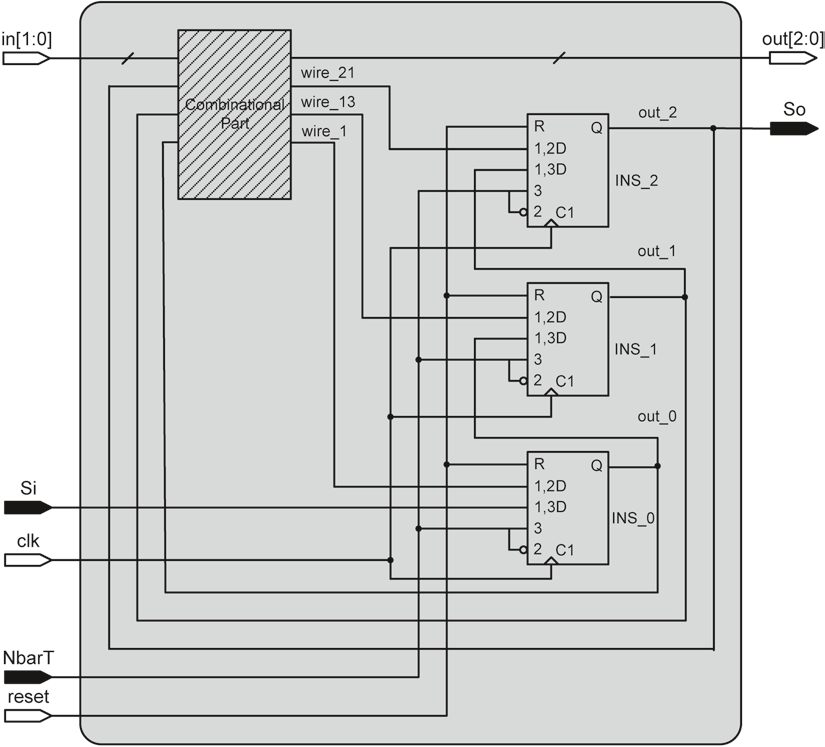
\includegraphics[width=0.7\textwidth]{images/MultipleParallelScanChains.png}
    \caption{\textit{Chuỗi quét đa luồng song song (Multiple parallel scan chains)}}
\end{figure}

Thời gian cho một lần kiểm thử với số lượng flip-flop là $N_{FF}$ có chu kỳ là $N_{FF} + 1$. Tổng thời gian kiểm tra cho $N_{Test}$ vector sẽ là:
\[ T_{test} = N_{Test} \times (N_{FF} + 1) + N_{FF} \]

% 5.2
\subsubsection{Thiết kế Quét qua Thanh ghi Bóng (Shadow Register DFT)}
Shadow Register là một dạng thiết kế lưu trữ song song cực kỳ thông minh trong việc giảm độ trễ (delay) hoặc phục vụ quá trình Capture lại trạng thái hệ thống mà không làm gián đoạn luồng dữ liệu (Data Path). 

Một thanh ghi "Bóng" (Shadow) được đặt sát các Master-FF của hệ thống. Trong quá trình Normal Mode, dữ liệu chạy mượt mà không vướng MUX. Khi có xung nhịp TestClock chuyên biệt, hệ thống "chụp" toàn bộ trạng thái Master-FF đẩy vào Shadow Register để chuẩn bị dịch ra ngoài theo chuỗi Serial (Observability). Kỹ thuật này đổi lấy diện tích Gated to hơn nhưng Performance tăng lên cực đại.

% 5.3
\subsubsection{Phương pháp Quét Cục bộ (Partial Scan Methods)}
Chèn 100\% Flip-Flop nội bộ (Full Scan) thường gây lãng phí từ $10\% - 20\%$ tài nguyên Area/Power của Chip. Để cân bằng (Tradeoff), kỹ thuật Partial Scan chỉ lựa chọn chọn lọc (Selective Insertion) những Flip-flop khó quan sát nhất, hay bẻ gãy một cách tinh tế các vòng lặp phản hồi hóc búa để kết lại thành Scan Chain ngắn gọn. Phương pháp này đòi hỏi công cụ ATPG phải có khả năng xử lý Test Pattern phức tạp hơn trên các phần mạch rải rác.

% 5.4
\subsubsection{Thiết kế Quét Đa luồng (Multiple Scan Design)}
Sự trả giá quá lớn cho thời gian của Single Scan dẫn đến nguyên lý đa chuỗi (Multiple Scans). Hệ thống sẽ tách chuỗi dài ra thành thành $k$ nhánh nhỏ chạy song song với nhau. Do đó, mỗi nhánh sẽ có độ dài $N'_{FF} = \lceil N_{FF} / k \rceil$. Thời gian kiểm tra nay giảm đi $k$ lần, chỉ còn:
\[ T_{test\_multiple} = N_{Test} \times (N'_{FF} + 1) + N'_{FF} \]

Ví dụ với vi xử lý nhỏ (CPU Adding Machine), chia ra 3 luồng riêng rẽ:
\begin{enumerate}
    \item \textbf{Chuỗi 1: Instruction Register (IR):} \texttt{ir\_Si} $\rightarrow$ \texttt{ir\_So} (8 Flip-flops)
    \item \textbf{Chuỗi 2: Accumulator (AC):} \texttt{ac\_Si} $\rightarrow$ \texttt{ac\_So} (8 Flip-flops)
    \item \textbf{Chuỗi 3: Program Counter (PC):} \texttt{pc\_Si} $\rightarrow$ \texttt{cntrl\_So} (8 Flip-flops)
\end{enumerate}

\begin{figure}[H]
    \centering
    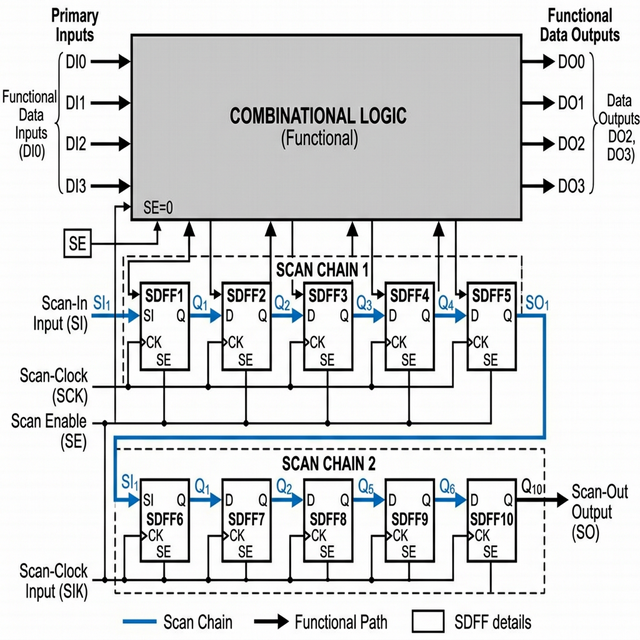
\includegraphics[width=0.7\textwidth]{images/scan_chain.png}
    \caption{\textit{Kết nối đa chuỗi quét song song cho cỗ máy cộng Adding Machine}}
\end{figure}

Việc sử dụng 3 cụm quét song song yêu cầu 3 chân lấy tín hiệu vào nối tiếp (Si), 3 chân xuất (So), và một chân \texttt{NbarT} điều khiển chế độ dung chung. Tester phải tách mảng data test ra 3 chùm (mỗi chùm 8 bits) và đẩy vào \texttt{ir\_Si}, \texttt{ac\_Si}, \texttt{pc\_Si} song song trên từng clock cạnh nhịp. Tương tự, bộ thu nhận mẫu từ 3 cổng xuất (\texttt{ir\_So}, \texttt{ac\_So}, \texttt{cntrl\_So}) cần phân tích dữ liệu gộp mảng theo đúng thứ tự rồi đem so sánh với kỳ vọng. Khối lệnh nạp dữ liệu cũng giảm số lần lặp đi từ 24 chu kì xuống 8 chu kì.

\begin{figure}[H]
    \centering
    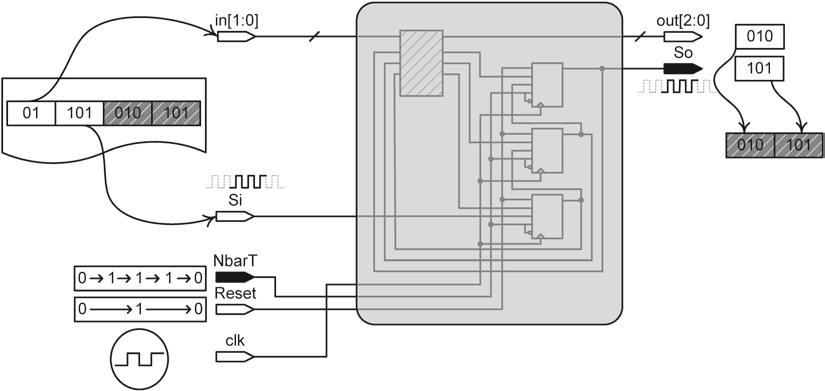
\includegraphics[width=0.7\textwidth]{images/FullScanAddingMachineVirtualTester.png}
    \caption{\textit{Trình kiểm thử ảo Full scan cho Adding Machine}}
\end{figure}

% 5.5
\subsubsection{Các Thiết Kế Quét Khác (Other Scan Designs)}
Bên cạnh cấu trúc Shift-register Chain, mảng vi mạch đặc biệt yêu cầu các hệ kiến trúc khác:
\begin{itemize}
    \item \textbf{Random Access Scan (Quét Truy Cập Ngẫu Nhiên):} Xây dựng mảng Flip-Flop y hệt kiến trúc SRAM tĩnh bằng bộ MUX ma trận. Cho phép kích hoạt riêng lẻ bất cứ Flip-flop trạng thái nào thông qua địa chỉ (Address Decoder) mà không cần phải shift tốn hàng ngàn chu kỳ.
\end{itemize}
